\chapter{Public-Data Transfer and Image-Only Deep Learning}\label{ch:5}

This chapter adds external knowledge: 4,827 ECG--echocardiography pairs from the public EchoNext data \cite{ref23}, redrawn in the hospital printout format. The EchoNext file was split by patient into 3,853 training and 974 test ECGs. Under the data-use agreement the EchoNext data stay on the owner's computer, so every model that uses them was trained there, under the same rule as every other model: until its training accuracy reached (nearly) 100 \%.

\section{EchoNext in the printout format}\label{sec:5.1}

\begin{table}[htbp]
\caption{Models trained only on EchoNext (every model trained to (nearly) 100 \% training accuracy, on the owner's computer) and applied to the 837 hospital ECGs; sorted by training accuracy. Training and validation accuracy on EchoNext; hospital accuracy with only the decision thresholds tuned on the hospital training folds (harmonised / plain input where both were run). $^{\ddagger}$ Two-class task (Mild against Moderate). Numbers as reported by that run.}\label{tab:5.1}
\footnotesize\setlength{\tabcolsep}{3pt}
\begin{tabular}{>{\raggedright\arraybackslash\hspace{0pt}}p{\dimexpr 0.420\linewidth-2\tabcolsep\relax}>{\raggedright\arraybackslash\hspace{0pt}}p{\dimexpr 0.160\linewidth-2\tabcolsep\relax}>{\raggedright\arraybackslash\hspace{0pt}}p{\dimexpr 0.180\linewidth-2\tabcolsep\relax}>{\raggedright\arraybackslash\hspace{0pt}}p{\dimexpr 0.240\linewidth-2\tabcolsep\relax}}
\toprule
\textbf{Model} & \textbf{Training acc. (EchoNext)} & \textbf{Validation acc. (EchoNext)} & \textbf{Hospital held-out acc.} \\
\midrule
EN-MiMo-GBM (Mild vs Moderate)$^{\ddagger}$ & 1.000 & 0.694 & 0.586 \\
EN-MiMo-LR (Mild vs Moderate)$^{\ddagger}$ & 1.000 & 0.604 & 0.577 \\
EN-gbm-X & 1.000 & 0.756 & 0.539 \\
EN-gbm & 1.000 & 0.756 & 0.522 / 0.522 \\
EN-cls & 1.000 & 0.663 & 0.479 \\
PIX-ZS (pixel CNN, EchoNext printouts) & 0.999 & 0.725 & 0.505 \\
EN-cls-all & 0.999 & 0.673 & 0.490 / 0.464 \\
EN-mu-mid & 0.999 & 0.463 & 0.409 \\
EN-cls-all-X & 0.996 & 0.694 & 0.497 \\
PIX-ZS-band (pixel CNN, EF bands) & 0.929 & 0.642 & 0.492 \\
EN-band-all & 0.820 & 0.525 & 0.458 / 0.465 \\
EN-band & 0.781 & 0.520 & 0.479 \\
\bottomrule
\end{tabular}
\end{table}


EchoNext waveforms were converted back to millivolts, resampled to 500 Hz, harmonised to the hospital baseline and cut into the printout's 2.5-s windows. The converted signals behave like the hospital's: heart-rate agreement $r=0.96$, QRS duration 82 against 82 ms and QTc 415 against 416 ms. Models trained only on EchoNext were then applied to the hospital printouts. \textbf{Transfer result.} The EchoNext-trained models fit their EchoNext training data almost perfectly (0.78--1.00) and reach 0.46--0.76 on EchoNext ECGs they have not seen (Table~\ref{tab:5.1}). Without any hospital training of the model, and with only its decision thresholds tuned on the hospital training folds, the best of them, LightGBM on the extended features (EN-gbm-X), reaches \textbf{0.539} four-class accuracy on the hospital printouts, and the two-class Mild-against-Moderate model 0.586.

\section{Pruned ensembles of all image-derived models}\label{sec:5.2}

\begin{table}[htbp]
\caption{Ensembles of image-derived members (837 ECGs, development cross-validation, corrected 95 \% CI), every member trained to (nearly) 100 \% training accuracy and every selection and meta-learner chosen inside the training folds; sorted by training accuracy. Ensembles with EchoNext members were run on the owner's computer.}\label{tab:5.2}
\footnotesize\setlength{\tabcolsep}{3pt}
\begin{tabular}{>{\raggedright\arraybackslash\hspace{0pt}}p{\dimexpr 0.470\linewidth-2\tabcolsep\relax}>{\raggedright\arraybackslash\hspace{0pt}}p{\dimexpr 0.140\linewidth-2\tabcolsep\relax}>{\raggedright\arraybackslash\hspace{0pt}}p{\dimexpr 0.140\linewidth-2\tabcolsep\relax}>{\raggedright\arraybackslash\hspace{0pt}}p{\dimexpr 0.250\linewidth-2\tabcolsep\relax}}
\toprule
\textbf{Ensemble} & \textbf{Members} & \textbf{Training acc.} & \textbf{Held-out acc. [95 \% CI]} \\
\midrule
ENH-vote, image-only members & 6 & 1.000 & 0.549 [0.513, 0.585] \\
C3 (Phase 5 selected model, reads the printed header) & 3 & 0.995 & 0.533 [0.496, 0.569] \\
ULT-stack, image-only members & 10 + EF & 0.794 & 0.537 [0.500, 0.574] \\
SUPER: greedy member selection, logistic meta-learner (with EchoNext members) & greedy & 0.790 & 0.552 [0.507, 0.596] \\
SUPER-TOP10-ORD, hospital-trained members only & 10 & 0.783 & 0.539 [0.509, 0.570] \\
SUPER-TOP10-ORD: ten best members, ordinal meta-learner (with EchoNext members) & 10 & 0.748 & 0.558 [0.530, 0.587] \\
STAGED-4: extended pool, staged meta-learner (with EchoNext members) & 10 & 0.722 & 0.548 [0.516, 0.581] \\
\bottomrule
\end{tabular}
\end{table}


Image-derived members were pooled: ECGFounder heads, the ENH and ULT members, tabular feature models, the EF band model and the EchoNext-trained models. Inside every training fold, members were selected either greedily (gain $\ge0.002$, at most 10 members) or as the ten best single members (TOP10), and combined by a logistic, staged (STAGED-4: Normal / middle / Severe, then Mild against Moderate) or ordinal (Frank--Hall) meta-learner (Table~\ref{tab:5.2}). The best ensemble, SUPER-TOP10 with the ordinal meta-learner, reaches \textbf{0.558} [0.530, 0.587]; the greedy ensemble reaches 0.552 and the staged ensemble \textbf{0.548}. Without the EchoNext members the same recipe gives 0.539, so the public data add about two points. Because the meta-learners are fitted on out-of-fold member outputs, the ensembles reach only 0.72--0.79 training accuracy, although nearly every member fits its own training folds perfectly.

\section{Additional features for Mild and Moderate}\label{sec:5.3}

Seventy-three further features targeted the Mild and Moderate classes: repolarisation heterogeneity (TCRT, T-wave morphology dispersion, T complexity, non-dipolar residuum), QT dispersion, the QT variability index and per-lead R amplitude ratios. The strongest single markers were TCRT (AUROC 0.738 for Normal against reduced EF) and the lead I R ratio (0.731). They were added as members of the extended ensemble pool (X), which gave the best staged model.

\section{Image-only pixel models trained on EchoNext printouts}\label{sec:5.4}

\begin{figure}[htbp]
\centering
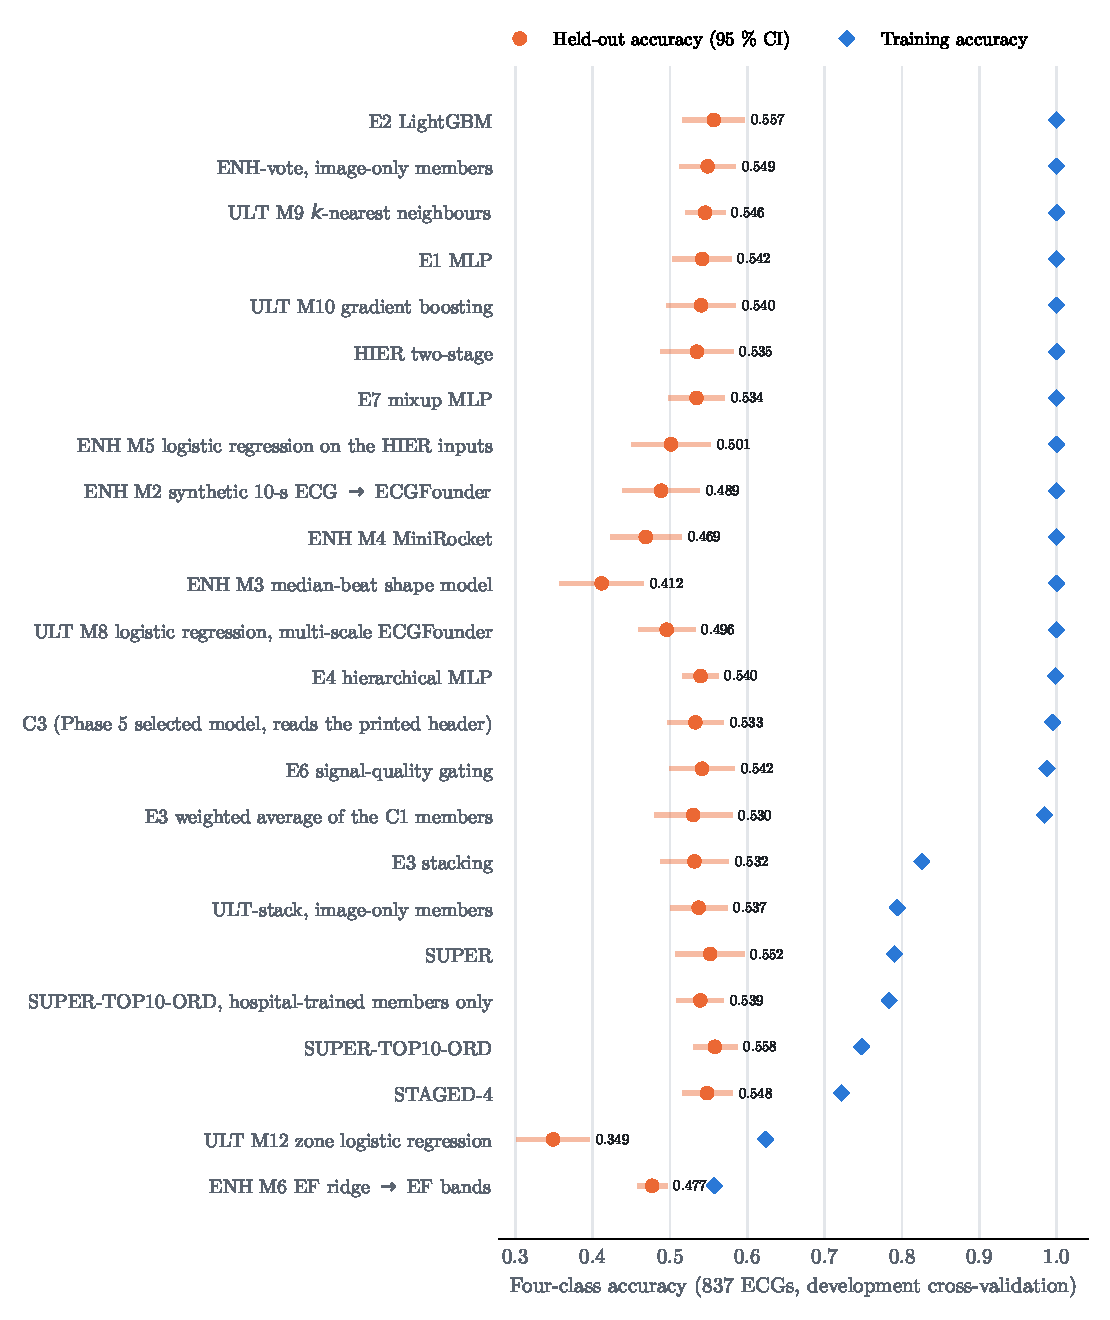
\includegraphics[width=0.91\linewidth,height=0.80\textheight,keepaspectratio]{figures/fig_5_1}
\caption{Ensembles and variants after training to (nearly) 100 \% training accuracy: held-out four-class accuracy with corrected 95 \% confidence intervals and training accuracy, sorted by training accuracy (837 ECGs, development cross-validation).}\label{fig:5.1}
\end{figure}

\begin{table}[htbp]
\caption{Pixel models that read the page image directly, every network trained to (nearly) 100 \% training accuracy; sorted by training accuracy. EchoNext accuracy: validation on EchoNext printouts.}\label{tab:5.3}
\footnotesize\setlength{\tabcolsep}{3pt}
\begin{tabular}{>{\raggedright\arraybackslash\hspace{0pt}}p{\dimexpr 0.420\linewidth-2\tabcolsep\relax}>{\raggedright\arraybackslash\hspace{0pt}}p{\dimexpr 0.120\linewidth-2\tabcolsep\relax}>{\raggedright\arraybackslash\hspace{0pt}}p{\dimexpr 0.130\linewidth-2\tabcolsep\relax}>{\raggedright\arraybackslash\hspace{0pt}}p{\dimexpr 0.120\linewidth-2\tabcolsep\relax}>{\raggedright\arraybackslash\hspace{0pt}}p{\dimexpr 0.210\linewidth-2\tabcolsep\relax}}
\toprule
\textbf{Model} & \textbf{Training acc.} & \textbf{EchoNext valid. acc.} & \textbf{Hospital acc.} & \textbf{Evaluation} \\
\midrule
EfficientNet-B0: hospital pages only & 1.000 & -- & 0.417 & fixed split, 168 validation ECGs \\
PIX-ZS: ResNet-18 trained on EchoNext printouts, applied to hospital pages & 0.999 & 0.725 & 0.505 & cross-validation (thresholds tuned) \\
ECGNet: hospital pages only & 0.999 & -- & 0.435 & fixed split, 168 validation ECGs \\
MobileNetV3-Large: hospital pages only & 0.999 & -- & 0.387 & fixed split, 168 validation ECGs \\
ResNet-18: hospital pages only & 0.997 & -- & 0.423 & fixed split, 168 validation ECGs \\
ConvNeXt-Atto: hospital pages only & 0.996 & -- & 0.345 & fixed split, 168 validation ECGs \\
PIX-ZS-band: the same network grading EF bands & 0.929 & 0.642 & 0.492 & cross-validation (thresholds tuned) \\
\bottomrule
\end{tabular}
\end{table}


Pixel CNNs read the page image directly. A ResNet-18 trained on EchoNext ECGs drawn as hospital printouts fits them almost perfectly (0.999) and reaches 0.725 on EchoNext test printouts. Applied to the hospital pages with only its thresholds tuned, it reaches 0.505, and its EF-band version 0.492 (Table~\ref{tab:5.3}). The CNNs trained on the hospital pages alone reach 0.345--0.435 on the fixed validation split, so the public printouts are the better teacher for a pixel network. Figure~\ref{fig:5.1} compares every ensemble and variant: all lie between 0.35 and 0.56 on held-out patients, whatever their training accuracy.
